In a complex system like the supercomputers we have today, the performance of Leaping Shadows is subject to both the hardware configuration, such as failure detection ability and the execution rate control mechanism, and software behavior, such as communication patterns and the amount of synchronization. 
It's extremely difficult for an analytical framework to precisely capture every details of Leaping Shadows when it runs in a real environment. Therefore, an executable prototype is necessary to prove its validity as well as measure its actual performance. 

As a proof of concept, we implement Leaping Shadows in a runtime library, referred to as rsMPI\footnote{The source code is available on BitBucket at git@bitbucket.org:Michael870/lsmpi.git}, for Message Passing Interface (MPI), which is the de facto programming paradigm for HPC. With the understanding that MPI standard keeps evolving to support new features and semantics, we focus on the most essential aspects and make srMPI MPI-1 compliant. %\footnote{rsMPI is developed in C programming language. Because MPI\_Request in Fortran has different type from C, rsMPI does not support MPI\_Isend() and MPI\_Irecv() that use MPI\_Request.}. 
Currently, rsMPI focuses on tolerating crash failures and associates one shadow process with each main process. %Collocation is used to achieve the desired execution rate of each shadow. 
With the rejuvenation technique introduced in Chapter~\ref{chapter:scale}, applying Leaping Shadows with dual modular redundancy minimizes the hardware and power costs, while being able to tolerate multiple failures. It is to be noted that, it is straightforward to extend this implementation to associate two shadows with each main, for the purpose of dealing with silent failures, as discussed in Chapter~\ref{chapter:sdc}. 


Instead of a full-feature MPI implementation, rsMPI library is designed to be a separate layer between MPI and user application, and it uses function wrappers on top of the MPI profiling hooks to intercept every MPI call. This is similar to the rMPI and redMPI implementations~\cite{ferreira_sc_2011,fiala_2012_sdc}. There are three benefits for this choice: 1) we can save tremendous time and efforts of rebuilding MPI from scratch; 2) we can take advantage of existing MPI performance optimization that numerous researches have spent years on, such as leveraging Remote Directory
Memory Access (RDMA) and OS bypass~\cite{woodall2006high}; and 3) the library is portable across all MPI implementations. 
When linked to an MPI application, rsMPI transparently spawns the shadow processes at the initialization phase, manages the coordination between main and shadow processes during execution, and guarantees order and consistency for messages and non-deterministic events.
%Once completed, users should be able to link to the library without any change to existing codes. 

%Currently, rsMPI focuses on tolerating crash failures and associates one shadow process with each main process. With the rejuvenation technique introduced in Chapter~\ref{chapter:scale}, applying Leaping Shadows with double modular redundancy minimizes the hardware and power costs while being able to tolerate multiple failures. It is to be noted that, it is straightforward to extend this implementation to associate two shadows with each each main, for the purpose of dealing with silent failures, as discussed in Chapter~\ref{chapter:sdc}. To achieve the desired execution rates for shadow processes, rsMPI uses shadow collocation, since this further reduces the hardware and power costs.

To avoid the drawbacks of DVFS, current rsMPI applies collocation to achieve the desired execution rates for the shadows. 
While each main executes on a separate processor at the maximum rate for HPC's throughput consideration, shadows are configured to collocate and execute at a slower rate based on a user configuration file. According to the user-provided number of processes and collocation ratio, rsMPI generates an MPI rankfile and provides it to the MPI runtime to control the process to processor mapping. Note that rsMPI always maps the main and shadow of a same task onto different nodes. This is required to prevent a fault on one node from affecting  both a main and its associated  shadow.


Despite the overview of the rsMPI library above, many challenges lie in efficiently integrating MPI with Leaping Shadows to support fault tolerance with high performance. One challenge is the preservation of the rich communication semantics in MPI standard. To be MPI-1 compliant, rsMPI needs to support both blocking and non-blocking point-to-point communications and blocking collective communications. A second challenge lies in coordination between the main and shadow process, in order to correctly terminate, carry out leaping, and perform failure recovery. Another challenge is that state consistency between mains and shadows needs to be maintained at all times. Last but not least, the side effects of divergence need to be addressed. %Specifically, there shall be no message buffer overflow; and the slower shadows shall not impact the performance of mains.
The following sections discuss solutions to the above challenges by presenting the rsMPI implementation details. 

\section{Function Wrappers}

As illustrated in Figure~\ref{fig:layer_arch}, rsMPI is positioned between the MPI runtime layer and the user application layer. Externally, rsMPI a library of function wrappers, one for each MPI primitive. As a result, user applications can be linked to rsMPI without modification to use MPI functions. When the user application makes an MPI function call, rsMPI library intercepts this call to enforce the Leaping Shadows logic. Internally, rsMPI uses the original MPI procedures by interacting with the MPI profiling interface. For example, to hide the existence of shadows from the user application, rsMPI adds a wrapper for the MPI\_Comm\_size() function, which is to retrieve the number of processes (i.e., MPI ranks) in an MPI communicator. When the user application calls MPI\_Comm\_size(), rsMPI internally calls PMPI\_Comm\_size() using the MPI profiling interface to retrieve a \textit{size}, counting both mains and shadows. Then rsMPI returns \textit{size/2} to the above application, giving an illusion that the same number of processes are launched. This is illustrate in Figure~\ref{fig:layer_arch_22}.


\begin{figure}[!h]
  \begin{center}
  	\subfigure[Position of the rsMPI library in software stack.]
		{
			\label{fig:layer_arch_11}
      		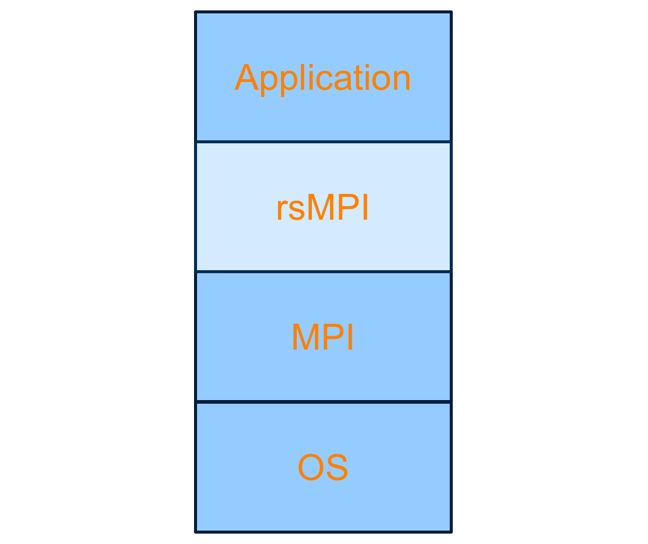
\includegraphics[width=0.45\columnwidth]{Figures/layer_arch_11}
      	}
  	\subfigure[Example of MPI\_Comm\_size() function call.]
		{
			\label{fig:layer_arch_22}
      		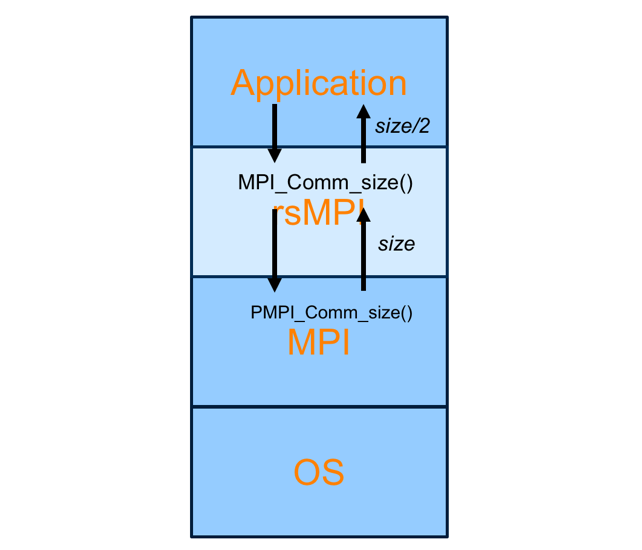
\includegraphics[width=0.45\columnwidth]{Figures/layer_arch_22}
      	}
  \end{center}
  \caption{rsMPI is inserted between the MPI and application layers to intercept MPI calls from the above application.}
  \label{fig:layer_arch}
\end{figure}

A static mapping between rsMPI ranks and application-visible MPI ranks is maintained so that each process can retrieve its identity. For example, if the user specifies $N$ ranks to launch, rsMPI will automatically translate it into $N + N$ ranks\footnote{This ignores the ranks for coordinator processes to be discussed later.}, with the first $N$ ranks being the mains, and the next $N$ ranks being their associated shadows in the corresponding order. By maintaining this main to shadow mapping, rsMPI guarantees that each process, whether main or shadow, gets its correct execution path. 
This logic is enforced by wrapping the MPI\_Comm\_rank() function. %so that each process (main or shadow) gets its correct execution path.
The wrappers for the MPI communication primitives will be discussed in the next section, where we introduce the consistency protocols.

\section{Message Passing and Consistency}
\label{sec:msg_consistency}
State consistency between mains and shadows is required both during normal execution and following a failure to leap-forward the shadows. 
Specifically, rsMPI needs to maintain sequential consistency so that each shadow sees the same message order and operation results as its main. 
Instead of having two parallel replica groups in which main communicates with main and shadow communicates with shadow~\cite{ferreira_sc_2011}, we choose to let the mains forward each message to the shadows. This allows us to speed up a single lagging shadow when a main fails. At the same time, the shadows are suppressed from sending out messages. As a consequence, two consistency protocols are explored, as depicted in Figure~\ref{fig:cons_protocol}. In the sender-forwarding protocol, as shown in Figure~\ref{fig:cons_protocol_1}, each main sender is responsible for forwarding each application message to the shadow of the receiver. In the receiver-forwarding protocol, as shown in Figure~\ref{fig:cons_protocol_2}, the main receiver is responsible for forwarding each received message to its associated shadow. 
%Instead of having two parallel replica groups in which main communicates with main and shadow communicates with shadow~\cite{ferreira_sc_2011}, we choose to let the mains forward each message to the shadows. This allows us to speed up a single lagging shadow when a main fails. 
%At the same time, the shadows are suppressed from sending out messages. 
We assume that two copies of the same message are sent in an atomic manner.

\begin{figure}[!t]
  \begin{center}
  	\subfigure[Sender-forwarding protocol.]
		{
			\label{fig:cons_protocol_1}
      		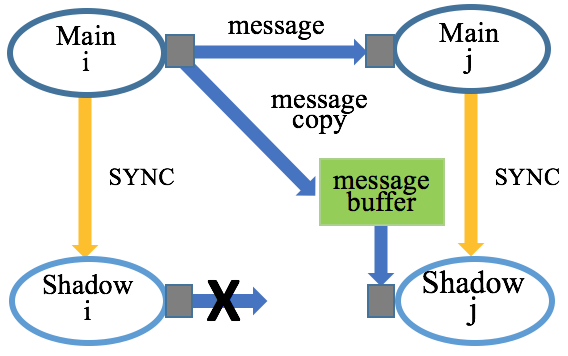
\includegraphics[width=0.45\columnwidth]{Figures/cons_protocol_1}
      	}
  	\subfigure[Receiver-forwarding protocol.]
		{
			\label{fig:cons_protocol_2}
      		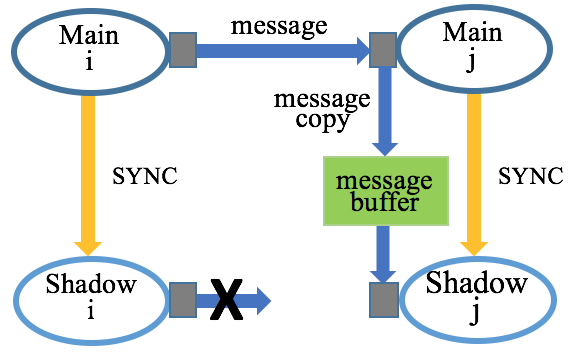
\includegraphics[width=0.45\columnwidth]{Figures/cons_protocol_2}
      	}
  \end{center}
  \caption{Consistency protocols for rsMPI.}
  \label{fig:cons_protocol}
\end{figure}



For MPI point-to-point communication routines, we add wrappers to implement the above consistency protocols. For sending functions, such as MPI\_Send() and MPI\_Isend(), the sender-forwarding protocol requires the main to duplicate the message, while in the receiver-forwarding protocol the main just does the normal sending. Again, the shadow is suppressed from sending, in both protocols. For receiving functions, such as MPI\_Recv() and MPI\_Irecv(), the sender-forwarding protocol requires that both the main and the shadow do one receiving from the main process at the sending side. In the receiver-forwarding protocol, MPI\_Recv() is modified such that the main performs a receiving followed by a sending to forward the message, and the shadow receives from its own main. For MPI\_Irecv(), it is slightly different that message forwarding is moved to MPI\_Test() and MPI\_Wait(), so that the message is assured to have arrived.

Collective communications, such as MPI\_Bcast() and MPI\_Allreduce(), are also supported in srMPI. To prevent the mains from slowing down by the shadows due to the synchronous semantic of collective communication, rsMPI maintains communicators that only contain the mains, and calls the original MPI function among the mains to perform a collective communication. Since the original MPI collective function is used, rsMPI automatically benefits from the optimization that has been put into the collective communications, such as~\cite{thakur2005optimization}. To keep the shadows consistent, results, if any, are forwarded from mains to shadows, so that shadows do not need to perform collective operation.
%, while the receiver-forwarding protocol changes the main to perform a receiving followed by a sending, and modifies the shadow to receive from its own main. 
%Collective communication in rsMPI uses point-to-point communication in a binomial tree topology, which demonstrates excellent scalability.

Assuming that only MPI operations can introduce non-determinism, the SYNC message shown in Figure~\ref{fig:cons_protocol} is used to enforce consistency when necessary. For example, under the sender-forwarding protocol MPI\_ANY\_SOURCE receiving may result in different message orders between a main and its shadow. To address this issue, we serialize the receiving of MPI\_ANY\_SOURCE messages by having the main finish the receiving and then use a SYNC message to forward the message source to its shadow, which then performs a normal receiving from the specific source. Other operations, such as MPI\_Wtime() and MPI\_Probe(), require both protocols to use the SYNC messages. Similar to MPI\_ANY\_SOURCE receiving, they are dealt with by forwarding each result from a main to its associated shadow.

\begin{table}[!h]
\caption{Comparison between sender-forwarding protocol and receiver-forwarding protocol. $N$ is the number of application message. $D$ is the number of non-deterministic event. $P$ is the number of process.}
\centering
\begin{tabular}{|c | c | c |}
\hline 
 & Sender-forwarding  & Receiver-forwarding  \\
\hline \hline 
Number of application message  & $2N$ & $2N$ \\
\hline
Number of SYNC message & $D$ &  $\le D$ \\
\hline
Shadow blocks main & Possible & Possible \\
\hline
Number of socket connection & $P^2$ & $P$ \\
\hline
Communication optimization & Hard & Easy \\
\hline
\end{tabular}
\label{tbl:cons_protocol_comp}
\end{table}

From the above analysis, we already see differences between the sender-forwarding protocol and the receiver-forwarding protocol. When deployed, they are expected to have further disparity on the cost and performance. 
A more detailed comparison is given in Table~\ref{tbl:cons_protocol_comp}. If an MPI application sends $N$ messages, both protocols double the number of application messages to be sent. Also, in both protocols, a slower shadow may block a faster main when message is forwarded from the main to the shadow. Therefore, flow control and buffer management need to be considered (to be discussed in following section). As mentioned above, the receiver-forwarding protocol does not need SYNC message in the case of MPI\_ANY\_SOURCE receiving, thus requiring fewer SYNC messages than the number of non-deterministic event, $D$. Furthermore, assuming an all-to-all connection of $P$ processes, the sender-forwarding protocol implies $P^2$ socket connections between mains and shadows, while the receiver-forwarding protocol only requires $P$ connections. Lastly, since each shadow only communicates with its associated main under the receiver-forwarding protocol, it is easier to optimize communication via process to processor mapping. For example, a heuristic may be that each shadow is placed in the same rack as its main, but not on the same node. Given the advantages of the receiver-forwarding protocol, we focus on this protocol in the following discussion and performance evaluation.



\section{Coordination between Main and Shadow}
To facilitate the correct execution of all processes, rsMPI adds a coordinator process to each shadowed set. 
Coordinators do not execute user application code, but just wait for rsMPI defined control messages. When a control message arrives, the coordinator carries out a minimal amount of coordination work accordingly. There are three types of control messages: termination, failure, and leaping. They corresponds to three actions:
\begin{itemize}
  \item When a main process finishes, the coordinator in the shadowed set forces the associated shadow process to terminate immediately.
  \item When a main process fails, the coordinator speeds up the associated shadow by temporarily suspending the other collocated shadows, until the recovery is complete.
  \item When a main process initiates a failure-induced leaping, the coordinator triggers leaping at the associated shadow process.
\end{itemize}


To minimize resource usage, each coordinator is collocated with the shadows in the shadowed set. 
A coordinator performs  minimal work, as its main task is to simply handle incoming control messages.  As such, the impact of the coordinator on the execution rate of the collocated shadows is negligible. To separate control messages from data messages, rsMPI uses a dedicated MPI communicator for the control messages. This Control Communicator is created by the wrapper of the MPI\_Init() function. In addition, to ensure fast response and minimize the number of messages, coordinators also use OS signals to communicate with their collocated shadows. This is illustrated in Figure~\ref{fig:coordinator}, assuming a collocation ratio of 2.


\begin{figure}[!t]
  \begin{center}
      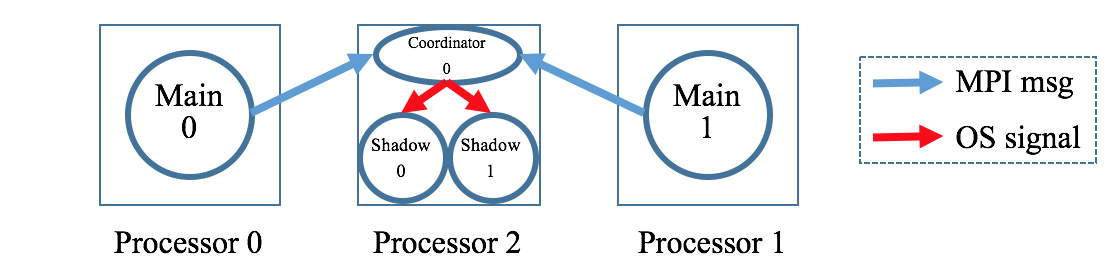
\includegraphics[width=\columnwidth]{Figures/coordinator}
  \end{center}
  \caption{A coordinator is added to each shadowed set. In this example, collocation ratio is 2 and each shadowed set contains 2 mains and 2 shadows.}
  \label{fig:coordinator}
\end{figure}



\section{Flow Control}
As discussed in Section~\ref{sec:msg_consistency}, rsMPI requires that mains forward application messages to shadows. Since the shadows are scheduled to execute at a slower rate than the mains, an implication is that a shadow may block a main when a message is forwarded from the main to the shadow. As a consequence, this may slow down the mains to proceed at the same rate as the shadows, significantly hurting the performance. 
This has been confirmed with our previous implementation where MPI communication is used for the forwarded messages. In many MPI implementations, two protocols are used for the communication. The eager protocol, which is used to transfer small messages, pushes the entire message to the receiver side regardless of the receiver being ready or not. In the rendezvous protocol, which is used for large messages, the sender is blocked until the receiver posts a matching receive. In order to prevent the shadows from blocking mains, lots of efforts need to be spent on tuning the eager threshold and buffer sizes for each application, not to mention that the eager threshold cannot be increased infinitely\footnote{In OpenMPI 1.10, the limit is 160 KB}. 
Due to message forwarding, another issue is that the divergence mentioned in Chapter~\ref{chapter:scale} will cause messages to accumulate at the shadow side, eventually leading to buffer overflow if no action is taken. With the previous implementation, we are not able to monitor or manipulate the buffers, which are managed by MPI runtime.

To simultaneously addressing these two issues, srMPI adopts a layered architecture, as shown in Figure~\ref{fig:flow_control}, to establish communication channels between mains and shadows with flow control capability. Under the receiver-forwarding protocol, each pair of main and shadow only requires one such channel. 

\begin{figure}[!t]
  \begin{center}
      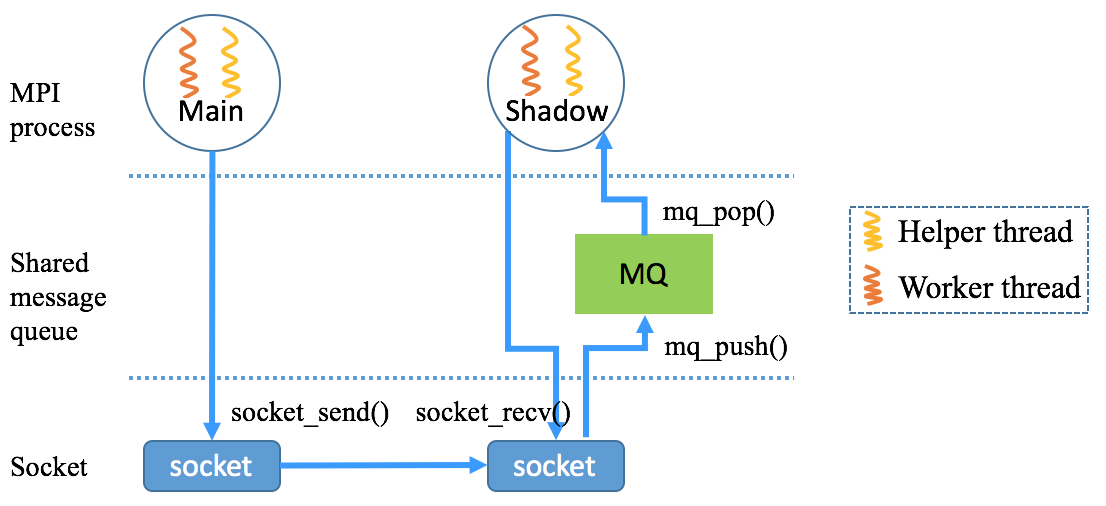
\includegraphics[width=\columnwidth]{Figures/flow_control}
  \end{center}
  \caption{A layered architecture for flow control in srMPI.}
  \label{fig:flow_control}
\end{figure}

At the lowest level, a socket connection to transfer application messages is established between each main and its associated shadow. When Remote Direct Memory Access (RDMA) is available, such as on the InfiniBand interconnects, srMPI uses the rsocket library, which provides a socket programming interface but internally uses RDMA for communication. Rather than copying data to the buffers of the operating system, RDMA enables the network adapter to transfer data directly from the main process to its shadow. The zero-copy networking feature of RDMA considerably reduces latency, thereby enabling fast transfer of data. When RDMA is not available, srMPI reverts back to TCP connections. 


At each shadow, a circular message queue, referred to as MQ, is implemented to store the messages that have been sent by main but not yet consumed by shadow. Similar to Linux socket buffer or Unix mbuf, MQ consists of two layers. The control layer contains fixed-length elements, each of which stores the meta-data of a message. The data layer is the actual buffer where variable-length message contents are stored. The control layer and data layer are connected via pointers. 

At the process level, a helper thread is added to each main and shadow process. The shadow helper thread is responsible for quickly responding to messages sent by the main on the socket connection, thus avoiding blocking the main. Every time there is a message, the shadow helper thread calls socket recv() to receive the message, and then stores it in its MQ. The main helper thread is mainly used to assist buffer-forced leaping. To avoid buffer overflow, a threshold is specified for MQ. If the threshold is reached, the shadow helper thread initiates a buffer-forced leaping, and notifies the corresponding main helper thread to participate in the leaping at the same time. After the buffer-forced leaping, obsolete messages in the MQ can be safely clearly. To minimize the impact of the helper threads on the performance of the compute threads, each helper thread is forced to relinquish CPU until a message arrives.





\section{Leaping}
With the focus on dealing with crash failures, three types of leaping are implemented in srMPI. To facilitate the following discussion, we summarize each leaping type along with the leap-provider and leap-recipient information in Table~\ref{tbl:srmpi_leaping}.

\begin{table}[!h]
\caption{Leaping types used in rsMPI.}
\centering
\begin{tabular}{|c | c | c |}
\hline 
Leaping type & Leap-provider  & Leap-recipient  \\
\hline \hline 
Failure-induced leaping & Main process & Shadow process \\
\hline
Buffer-forced leaping & Main process & Shadow process \\
\hline
Rejuvenation-induced leaping & Shadow process & Main process \\
\hline
\end{tabular}
\label{tbl:srmpi_leaping}
\end{table}


Checkpoint/restart requires each process to save its execution state, which can be used later to retrieve the state of the computation. 
Leaping, in all types, is similar to the checkpointing process, except that the state is directly transferred between a pair of main and shadow, thus requiring no additional storage space. 
To reduce the size of data involved in saving state, rsMPI uses a similar approach as application-level checkpointing~\cite{beguelin1997application,ni_2013_acr}, and requires users to identify necessary data as process state using the following API:

\begin{lstlisting}
void  leap_register_state(void *addr, int count, MPI_Datatype dt);
\end{lstlisting}

For each data set to be registered, three arguments are needed: a pointer to the memory address of the data set, the number of data items in the data set, and the datatype. 
Application developer could use domain knowledge to identify only necessary state data, or use compiler techniques to automate this process~\cite{Bronevetsky:09:Compiler}. 
Internally, rsMPI uses a linked list to keep track of all registered data. After each call of leap\_register\_state(), rsMPI adds a node to its internal linked list to record the three parameters. 
During leaping, the linked list is traversed to retrieve all registered data as the process state.

MPI communication channels are used in rsMPI to transfer process state. Although multiple data sets can be registered as a process' state, only a single message needs to be transferred, as MPI supports derived datatypes. To isolate state messages from application messages, rsMPI uses the Control Communicator to transfer process state.  
By using a coordinator to synchronize the leaping and relying on  MPI messages to rapidly transfer state, the overhead of leaping is minimized. 

To make sure a pair of main and shadow stay consistent after a leaping, not only user-defined states should be transferred, but also lower level states, such as program counter and message buffers, need to be correctly updated. Specifically, the leap-recipient needs to satisfy two requirements:  
1) Discard all obsolete messages, if any, after the leaping; 2) Resume execution at the same point as the leap-provider. We discuss our solutions below, under the assumption that the application's main body consists of a loop of iterations, which is true in most HPC applications.

In failure-induced and buffer-forced leaping, shadow is the leap-recipient. 
To correctly discard all obsolete messages at a shadow without throwing away useful ones, rsMPI requires every main and shadow maintain a counter for messages consumed. During leaping, the counter value at the main is transferred to the shadow, so that the latter knows how many messages to discard. Then the shadow can easily remove the obsolete messages because messages stored in MQ at the shadow are in the same order as those consumed by the main. In rejuvenation-induced leaping, the main is the leap-recipient, so there is no obsolete message to discard. 


To resume execution from the same point, we restrict leaping to always occur at specific points, and use an internal counter to make sure that both the leap-recipient and leap-provider start leaping from the same point. For example, when a main initiates a failure-induced leaping, the coordinator will trigger a rsMPI-defined signal handler at the associated shadow. The signal handler does not carry out leaping, but sets a flag for leaping and receives from its main a counter value that indicates the leaping point. %Then, the shadow will check the flag and compare the counter value at every possible leaping point. 
Only when both the flag is set and counter value matches will the shadow start leaping. In this way, it is guaranteed that after leaping the leap-recipient and leap-provider will resume execution from the same point. To balance the trade-off between implementation overhead and flexibility, we choose MPI receive operations as the only possible leaping points. 

\section{Evaluation}
We deployed rsMPI on a cluster of 30 nodes (600 cores) for testing and benchmarking. Each node consists of a 2-way SMPs with Intel Haswell E5-2660 v3 processors of 10 cores per socket (20 cores per node). Each node is configured with 128 GB of local memory. Nodes are connected via 56 GB/s FDR InfiniBand. To maximize the computing capacity, we used up to 20 cores per node.

Benchmarks from the Sandia National Lab Mantevo Project and NAS Parallel Benchmarks (NPB) are used, and we evaluated rsMPI with various problem sizes and number of processes. 
CoMD is a proxy for molecular dynamics application. MiniAero is an explicit unstructured finite volume code that solves the Navier-Stokes equations. Both MiniFE and HPCCG are unstructured implicit finite element codes, but HPCCG uses MPI\_ANY\_SOURCE receive operations and can demonstrate rsMPI's capability of handling non-deterministic events. LU, EP, and FT from NPB represent lower-upper Gauss-Seidel solver, embarrassingly parallel, and fast Fourier Transform, respectively. In addition, we choose the LULESH benchmark developed at the Lawrence Livermore National Lab, since it is a widely studied proxy application in DOE co-design efforts for exascale~\cite{LULESH2:changes}. These applications cover key simulation workloads and represent both different communication patterns and computation-to-communication ratios.

We also implemented checkpoint/restart to compare with rsMPI in the presence of failures. 
To be optimistic, we chose double in-memory checkpointing that is much more scalable than disk-based checkpointing~\cite{zheng_2004_ftccharm}. 
Same as leaping in rsMPI, our application-level checkpointing provides an API for process state registration. This API requires the same parameters, but internally, it allocates extra memory in order to store 2 checkpoints, one for the local process and one for a remote ``buddy" process. Another provided API is checkpoint(), which inserts a checkpoint in the application code. For fairness, MPI messages are used to transfer state between buddies.  
For both rsMPI and checkpoint/restart, we assume a 60 seconds rebooting time after a failure. All figures in this section show the average of 5 runs with the standard deviation.

\subsection{Measurement of Runtime Overhead}
\label{sec:runtime_overhead}
While the hardware overhead for rsMPI is straightforward (e.g., collocation ratio of 2 results in the need for 50\% more hardware), 
the runtime overhead due to the enforced consistency and coordination depends on applications. To measure this overhead we ran each benchmark application linked to rsMPI and compared the execution time with the baseline, in which each application runs with unmodified OpenMPI.

\begin{figure}[!t]
  \begin{center}
      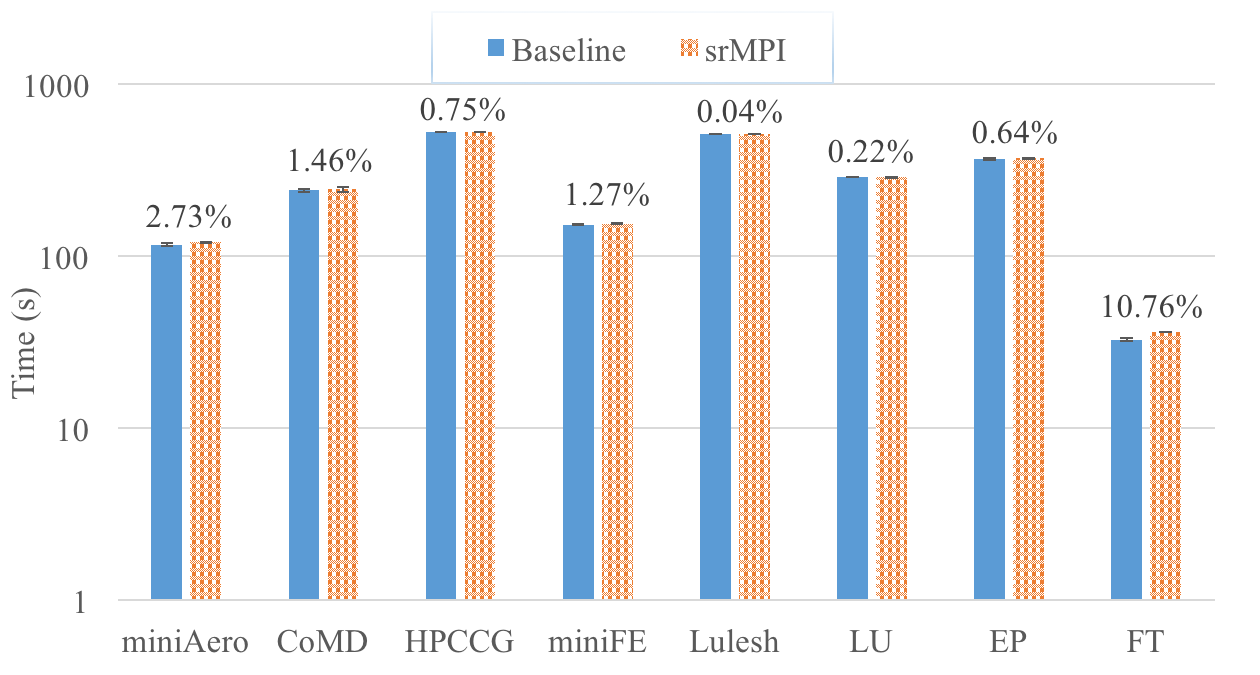
\includegraphics[width=0.6\columnwidth]{Figures/runtime_overhead}
  \end{center}
  \caption{Comparison of execution time between baseline and rsMPI. 256 application-visible processes, except 216 processes for LULESH. Collocation ratio is 2 for rsMPI.}
  \label{fig:runtime_overhead}
\end{figure}

Figure~\ref{fig:runtime_overhead} shows the comparison of the execution time for the 8 applications in the absence of faults. All the experiments are conducted with 256 application-visible processes, except that LULESH requires the number of processes to be a cube of an integer. When the baseline uses 256 MPI ranks, rsMPI uses 256 mains together with 256 shadows. The baseline execution time varies from seconds to 15 minutes, so we plotted the time in log-scale. 
From the figure we can see that rsMPI has comparable execution time to the baseline for all applications except FT. The reason for the exception is that FT uses a lot of broadcast, reduce, and all-to-all communication, and thus is heavily communication-intensive. This is verified by adding fake computation to the application and we can see an immediate drop of the overhead to negligible level. 
We argue that all-to-all communication applications like FT are not scalable, and as a result, they are not suitable for massively parallel HPC. 
For all others, the overhead varies from 0.04\% (LULESH) to 2.73\% (miniAero). Even for HPCCG, which uses MPI\_ANY\_SOURCE, the overhead is only 0.75\%, thanks to the flow control mechanism deployed in srMPI. 
Therefore, we conclude that rsMPI's runtime overheads are modest for applications that exhibit a fair communication-to-computation ratio.



\subsection{Scalability}

In addition to measuring the runtime overhead at a fixed process count, we also assessed the applications' weak scalability, which measures how the execution time varies with the number of processes for a fixed problem size per process.
Among the eight applications, HPCCG, CoMD, and miniAero allow us to configure the problem size for weak scaling test. The results for miniAero are similar to those of CoMD, so we only show the results for HPCCG and CoMD in Figure~\ref{fig:scalability}. 


\begin{figure}[!t]
	\begin{center}
		\subfigure[HPCCG weak scalability]
		{
			\label{fig:hpccg_weak}
			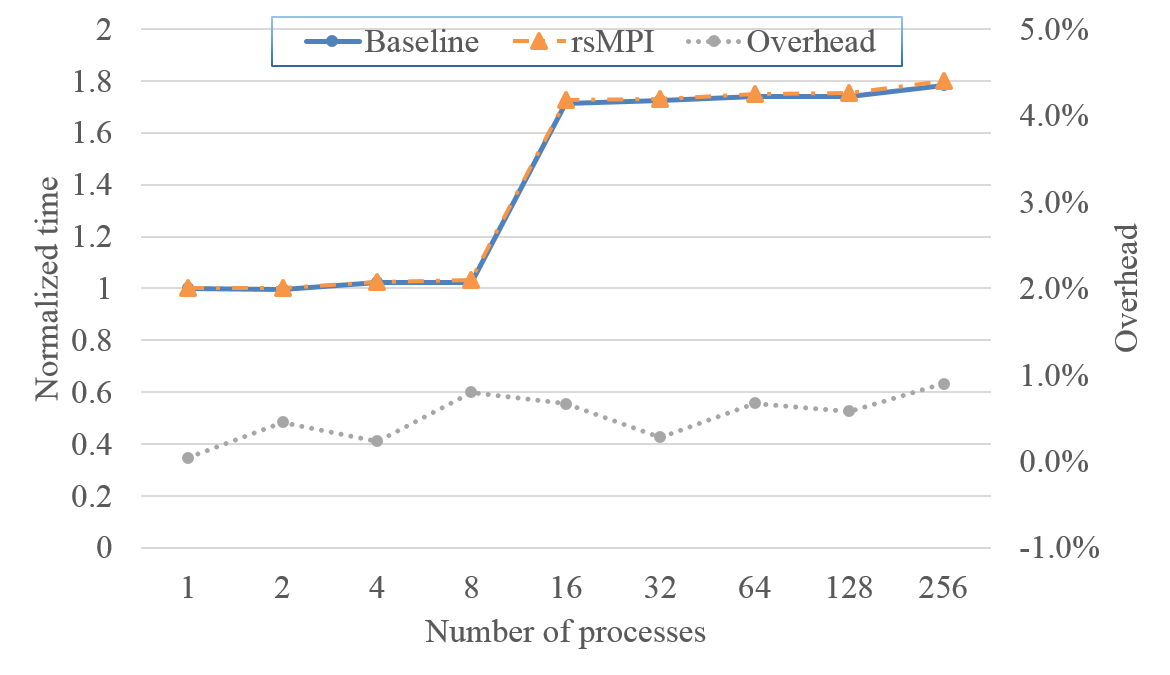
\includegraphics[width=0.45\columnwidth]{Figures/hpccg_weak}
		}
		\subfigure[CoMD weak scalability]
		{
			\label{fig:comd_weak}
			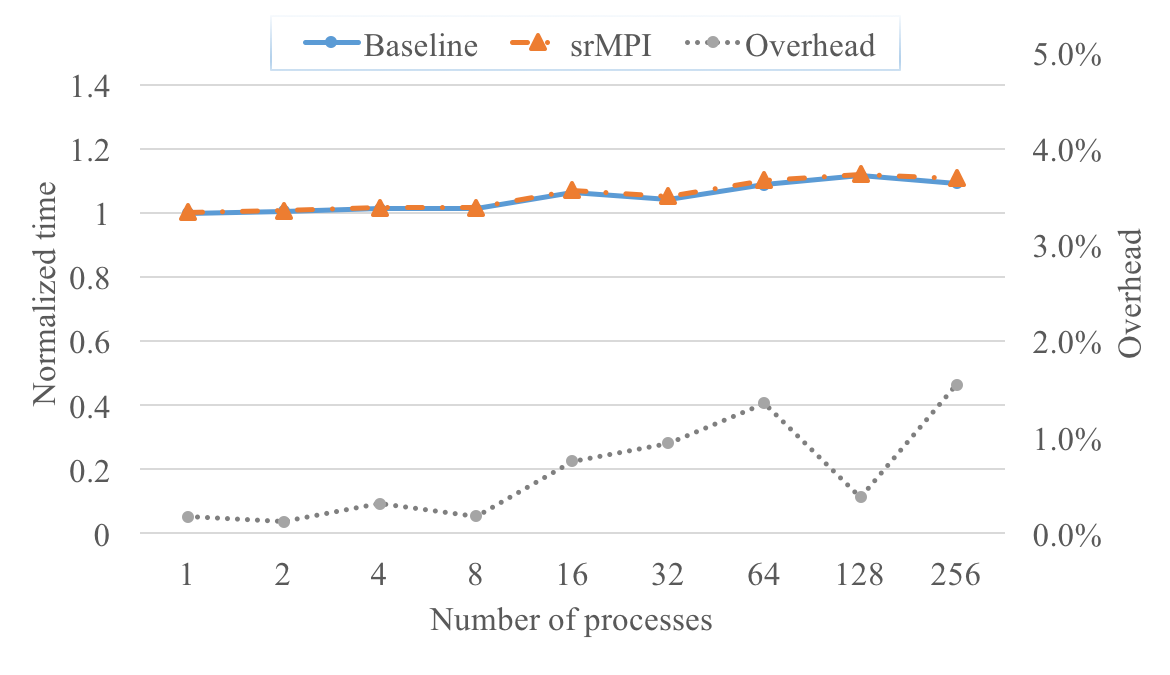
\includegraphics[width=0.45\columnwidth]{Figures/comd_weak}
		}
	\end{center}
	\caption{Weak scalability measurement with number of processes from 1 to 256. Collocation ratio is 2 for rsMPI. Time is normalized to that of the baseline with 1 process.}
	\label{fig:scalability}
\end{figure}

Comparing between Figure~\ref{fig:hpccg_weak} and Figure~\ref{fig:comd_weak}, it is obvious that HPCCG and CoMD have different weak scaling characteristics. While the execution time for CoMD increases by 9.3\% from 1 process to 256 processes, the execution time is almost doubled for HPCCG (1.78X). However, further analysis shows that the execution time increases by 67.4\% for HPCCG from 8 to 16 processes. We suspect that the results are not only affected by the scalability of the application, but also impacted by other factors, such as cache and memory contention on the same node, and network interference from other jobs running on the cluster. Note that each node in the cluster has 20 cores and we always use all the cores of a node before adding another node. Therefore, it is very likely that the node level contention leads to the substantial increase in execution time for HPCCG. The results from 16 to 256 processes show that both HPCCG and CoMD are weak scaling applications. 
%To predict the overhead at exascale, we applied curve fitting to derive the correlation between runtime overhead and the number of processes. At $2^{20}$ processes, it is projected that the overhead is 3.1\% for CoMD and 7.6\% for HPCCG. 

Similar to the results of the previous section, the runtime overhead for rsMPI is modest. The maximum overhead observed is 1.6\% when running CoMD with 256 processes. Excluding this case, the overhead is always below 1.0\%. To predict the overhead at exascale, we applied curve fitting to derive the correlation between runtime overhead and the number of processes. At $2^{20}$ processes, it is projected that the runtime overhead is 9.4\% for CoMD and 4.5\% for HPCCG. 


\subsection{Performance under Failures}
%The last set of experiments test rsMPI's capability of tolerating failures and evaluate its performance under various failures by comparing with checkpointing/restart. 

As one main goal of this work is to achieve fault tolerance, an integrated fault injector is required to evaluate the effectiveness and efficiency of rsMPI to tolerate failures during execution. 
To produce failures in a manner similar to naturally occurring process failures, the failure injector is designed to be distributed and co-exist with all rsMPI processes. Failure is injected by sending a specific signal to a randomly picked target process.

We assume that the underlying hardware platform has a Reliability, Availability and Serviceability (RAS) system that provides failure detection. In our test system, we emulate the RAS functionality by associating a signal handler with every process. The signal handler catches failure signals sent from the failure injector, and uses a rsMPI defined failure message via a dedicated communicator to notify all other processes of the failure\footnote{A similar idea has been tested in \cite{fang2017letgo}. By using GDB to intercept OS signals generated after a fault, a signal handler allows the failing process to continue work before crashing.}. 
To detect failure of another process, rsMPI receiving operation checks for failure messages before performing the actual receiving. 
Similar to ULFM~\cite{bland2013post}, a process in rsMPI can only detect failure when it posts an MPI receive operation. 

The first step was to test the effectiveness of leaping.  
Figure~\ref{fig:single_failure} shows the execution time of HPCCG with a single failure injected at a specific time, measured as a proportion of the total execution of the application, at an increment of 10\%.
The execution time is normalized to that of the failure-free baseline.   
The blue solid line and red dashed line represent rsMPI with collocation ratio of 2 and 4, respectively. For simplicity, they are referred to as rsMPI\_2 and rsMPI\_4 in the following text.  


\begin{figure}[!t]
  \begin{center}
      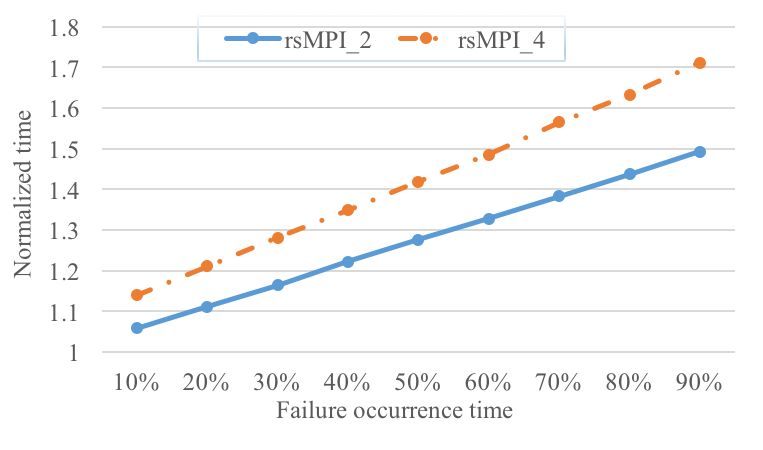
\includegraphics[width=0.6\columnwidth]{Figures/single_failure_srmpi}
  \end{center}
  \vskip -0.2in
  \caption{Execution time of HPCCG under rsMPI with a single failure injected at various time, normalized to that of the failure-free baseline.}
  \label{fig:single_failure}
\end{figure}

As shown in Figure~\ref{fig:single_failure}, rsMPI's execution time increases with the failure occurrence time, regardless of the collocation ratio. The reason is that recovery time in rsMPI is proportional to the amount of divergence between mains and shadows, which grows with the execution. 
Another factor that determines the divergence is the shadow's execution rate. The slower the shadows execute, the faster the divergence grows. As a result, rsMPI\_2 can recover faster than rsMPI\_4, and therefore achieves better execution time.



The results in Figure~\ref{fig:single_failure} suggests that rsMPI is better suited to environments where failures are frequent. 
This stems from the fact that, due to leaping, the divergence between mains and shadows is eliminated after every failure recovery. As the number of failure increases, the interval between failures decreases, thereby reducing the recovery time per failure.
To demonstrate the above analysis, we compare rsMPI with checkpoint/restart under various failure rates. 
To run the same number of application-visible processes, rsMPI needs more nodes than checkpoint/restart to host the shadow processes. 
For fairness, we take into account the extra hardware cost for rsMPI by defining the weighted execution time:
$$T_{weight} = T_e \times S_p,$$ where $T_e$ is the wall-clock execution time and $S_p$ is the projected speedup. For example, we measured that the speedup of HPCCG from 128 processes to 256 processes is 1.88, and rsMPI\_2 needs 1.5 times more nodes than checkpoint/restart, so the projected speedup is $1.5\times\frac{1.88}{2}=1.41$. Similarly, the projected speedup for rsMPI\_4 is $1.25\times\frac{1.88}{2}=1.17$.


%The buffer-forced leaping interval for an application is selected such that no buffer overflow at the shadows would take place. Therefore, the interval should vary from system to system and also depends on the application communication patterns. We assume checkpoint/restart has the same buffer pressure as it needs to perform message logging, so its checkpointing interval is selected based on the same metric as rsMPI. We evaluated rsMPI with 2 different collocation ratios, i.e., 2 and 4. When collocation ratio is 2, rsMPI uses 50\% more nodes than checkpoint/restart, and the execution rate of each shadow is roughly 50\% of the processor rate. Therefore, we set the checkpointing interval to be the same as the forced leaping interval for rsMPI. When collocation ratio is 4, rsMPI needs 25\% more nodes, and each shadow's rate is roughly 25\% of the processor rate. As a result, we loose the checkpointing interval to be twice of the forced leaping interval. 


In this analysis, we set the checkpointing interval to $0.1T$, where $T$ is the total execution time. To  both checkpoint/restart and rsMPI, we randomly inject over $T$ a number of faults, $K$, ranging from 1 to 30. This fault rate corresponds to a processor's MTBF of $NT/K$, where $N$ is the number of processors. That is, the processor's MTBF is proportional to the total execution time and the number of processors. For example, when using $256$ processors and executing for $1700$ seconds, injecting $10$ faults corresponds to a processor's MTBF of $12$ hours. However, 
when using a system of $64,000$ processors and executing over $4$ hours, injecting $10$ faults corresponds to a processor's MTBF of $3$ years.

Figure~\ref{fig:multiple_failure} compares checkpoint/restart and rsMPI, based on both wall-clock and weighted execution time. Ignoring the hardware overhead, Figure~\ref{fig:failures_time} shows that, in the failure-free case, checkpoint/restart slightly outperforms rsMPI. As the number of failures increases, however, rsMPI achieves significantly higher performance than checkpoint/restart. For example, when the number of failures is 20, rsMPI\_2 saves 33.4\% in time compared to checkpoint/restart. The saving rises up to 40.8\%, when the number of failures is increased to $30$. Compared to checkpoint/restart, rsMPI\_4 reduces the execution time by 33.1\% and 40.5\%, when the number of failures are 20 and 30, respectively. 

\begin{figure}[!t]
  \begin{center}
      \subfigure[Wall-clock execution time]
		{
			\label{fig:failures_time}
			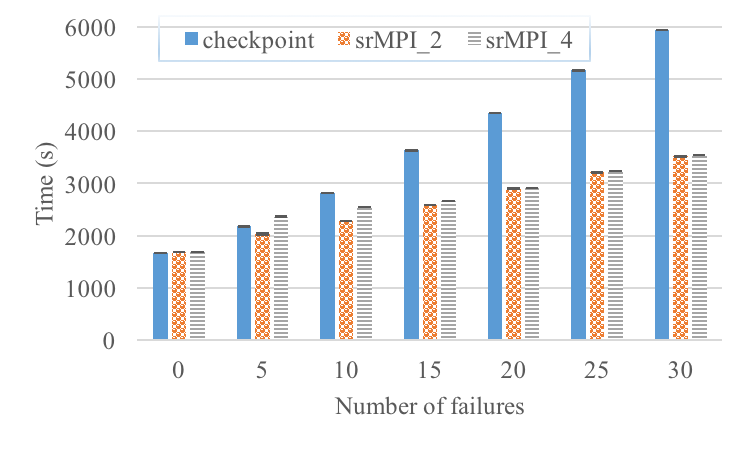
\includegraphics[width=0.45\columnwidth]{Figures/failures_time_srmpi}
		}
		\subfigure[Weighted execution time]
		{
			\label{fig:failures_ntime}
			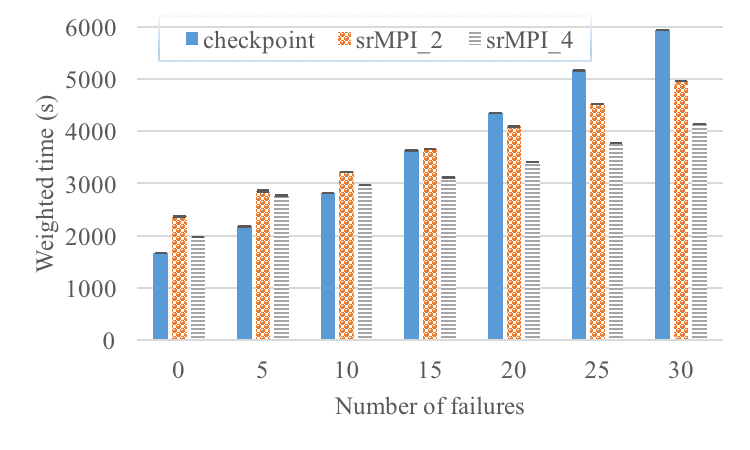
\includegraphics[width=0.45\columnwidth]{Figures/failures_ntime_srmpi}
		}
  \end{center}
  \caption{Comparison between checkpoint/restart and rsMPI with various number of failures injected to HPCCG. 256 application-visible processes, 10\% checkpointing interval.}
  \label{fig:multiple_failure}
\end{figure}


Careful analysis of Figure~\ref{fig:failures_time} reveals that, as the number of failures increases, checkpoint/restart and rsMPI exhibit different performance degradation. As expected, the execution time for checkpoint/restart increases proportionally with the number of failures. For rsMPI, however, the increase is sub-linear. This is due to fact that as more failures occur, the interval between failures is reduced, and as a result, the recovery time per failure is also reduced. 
Eventually, the constant rebooting time dominates the recovery overhead. This is the reason why the execution time of srMPI\_2 and srMPI\_4 tends to converge as the number of failure increases. 
%Although not shown in Figure~\ref{fig:failures_time}, rebooting time will eventually dominate the recovery time when more failures occur, resulting in a linear increase in execution time for rsMPI. This increase, however, occurs at a significantly slower rate than checkpoint/restart.

Incorporating hardware overhead, Figure~\ref{fig:failures_ntime} compares the weighted execution time between checkpoint/restart and rsMPI.  As expected, checkpoint/restart is better when the number of  failures is small (e.g., 5 failures).  When the number of failures increases,  however, checkpoint/restart loses its advantage quickly. At 30 failures, for example, rsMPI\_2 and rsMPI\_4 are 16.5\% and 30.4\% more efficient than checkpoint/restart, respectively.
Note that, when comparing rsMPI\_2 and rsMPI\_4, the former shows higher performance with respect to wall-clock execution time, while the latter is better with respect to weighted execution time. 

\section{Summary}
This chapter presents the details of a proof-of-concept implementation of Leaping Shadows in MPI, referred to as rsMPI. To ensure correct execution while maximizing performance, rsMPI consists of five building blocks: wrappers for MPI functions, consistency protocols to maintain sequential consistency and resolve non-determinism, main and shadow coordination mechanism, flow control algorithm with customized data structure, and an application-level leaping protocol. Based on shadow collocation, this implementation associates one shadow process with each main process to tolerate crash failures. By capturing the leaping (include failure-induced leaping, buffer-forced leaping, and rejuvenation-induced leaping) and rejuvenation techniques, rsMPI enables MPI applications to tolerate multiple failures with minimized hardware and power costs. 

With rsMPI, extensive experiments have been done to evaluate the performance of the Leaping Shadows fault tolerance model in real systems. To cover key HPC simulation workloads, we use benchmark applications that represent both different communication patterns and different computation-to-communication ratios. By comparing with the original OpenMPI library, we demonstrate that rsMPI has negligible runtime overheads when there is no failure. Also, we implement and compare to in-memory checkpoint/restart under various failure rates.
Experiment results show that rsMPI has a high potential in outperforming in-memory checkpoint/restart in both execution time and resource utilization, especially in failure-prone environments.




